\setcounter{figure}{0}

\section{7th May 2023: The New Jerusalem}
\subsection*{Text: Revelation 21:1-22:5}
  \begin{quote}
    [1] Then I saw a new heaven and a new earth, for the first heaven and the
    first earth had passed away, and the sea was no more. [2] And I saw the
    holy city, new Jerusalem, coming down out of heaven from God, prepared as
    a bride adorned for her husband. [3] And I heard a loud voice from the
    throne saying, “Behold, the dwelling place of God is with man. He will
    dwell with them, and they will be his people, and God himself will be
    with them as their God. [4] He will wipe away every tear from their eyes,
    and death shall be no more, neither shall there be mourning, nor crying,
    nor pain anymore, for the former things have passed away.”

    [5] And he who was seated on the throne said, “Behold, I am making all
    things new.” Also he said, “Write this down, for these words are
    trustworthy and true.” [6] And he said to me, “It is done! I am the Alpha
    and the Omega, the beginning and the end. To the thirsty I will give from
    the spring of the water of life without payment. [7] The one who conquers
    will have this heritage, and I will be his God and he will be my son. [8]
    But as for the cowardly, the faithless, the detestable, as for murderers,
    the sexually immoral, sorcerers, idolaters, and all liars, their portion
    will be in the lake that burns with fire and sulfur, which is the second
    death.”

    [9] Then came one of the seven angels who had the seven bowls full of the
    seven last plagues and spoke to me, saying, “Come, I will show you the
    Bride, the wife of the Lamb.” [10] And he carried me away in the Spirit
    to a great, high mountain, and showed me the holy city Jerusalem coming
    down out of heaven from God, [11] having the glory of God, its radiance
    like a most rare jewel, like a jasper, clear as crystal. [12] It had a
    great, high wall, with twelve gates, and at the gates twelve angels, and
    on the gates the names of the twelve tribes of the sons of Israel were
    inscribed—[13] on the east three gates, on the north three gates, on the
    south three gates, and on the west three gates. [14] And the wall of the
    city had twelve foundations, and on them were the twelve names of the
    twelve apostles of the Lamb.

    [15] And the one who spoke with me had a measuring rod of gold to measure
    the city and its gates and walls. [16] The city lies foursquare, its
    length the same as its width. And he measured the city with his rod,
    12,000 stadia. Its length and width and height are equal. [17] He also
    measured its wall, 144 cubits by human measurement, which is also an
    angel’s measurement. [18] The wall was built of jasper, while the city
    was pure gold, like clear glass. [19] The foundations of the wall of the
    city were adorned with every kind of jewel. The first was jasper, the
    second sapphire, the third agate, the fourth emerald, [20] the fifth
    onyx, the sixth carnelian, the seventh chrysolite, the eighth beryl, the
    ninth topaz, the tenth chrysoprase, the eleventh jacinth, the twelfth
    amethyst. [21] And the twelve gates were twelve pearls, each of the gates
    made of a single pearl, and the street of the city was pure gold, like
    transparent glass.

    [22] And I saw no temple in the city, for its temple is the Lord God the
    Almighty and the Lamb. [23] And the city has no need of sun or moon to
    shine on it, for the glory of God gives it light, and its lamp is the
    Lamb. [24] By its light will the nations walk, and the kings of the earth
    will bring their glory into it, [25] and its gates will never be shut by
    day—and there will be no night there. [26] They will bring into it the
    glory and the honor of the nations. [27] But nothing unclean will ever
    enter it, nor anyone who does what is detestable or false, but only those
    who are written in the Lamb’s book of life.

    [1] Then the angel showed me the river of the water of life, bright as
    crystal, flowing from the throne of God and of the Lamb [2] through the
    middle of the street of the city; also, on either side of the river, the
    tree of life with its twelve kinds of fruit, yielding its fruit each
    month. The leaves of the tree were for the healing of the nations. [3] No
    longer will there be anything accursed, but the throne of God and of the
    Lamb will be in it, and his servants will worship him. [4] They will see
    his face, and his name will be on their foreheads. [5] And night will be
    no more. They will need no light of lamp or sun, for the Lord God will be
    their light, and they will reign forever and ever.
  \end{quote}
\subsection*{Notes}
\begin{itemize}
  \item{God has promised to make everything new. This renewal promise is in
  the context of a covenant relationship, which is established with the
  covenant formula: ``I will be your God, you will be My people''. Today's
  text is the fulfilment of this renewal promise which God has made a long
  time ago (e.g in Ezekiel 37, in Jeremiah 29, etc).}
  \item{In today's text, we have mentions of a new heaven and a new earth.
  Yet from a secular perspective, people like Karl Marx have said that
  ``religion is the opium of the people'', because when people believe in a
  new heaven and new earth, it helps them escape the pain of the current
  earth. People like Karl Marx have been prophesied about in 2 Peter, as part
  of the group of scoffers who doubt Jesus' second coming. The new heaven and
  the new earth that will come down from heaven is God's doing, it is not our
  doing. Unlike the atheistic humanism of Marx, from the Christian
  perspective, only God can renew the creation. In a sense, we have a greater
  awareness of the problem of sin that plagues humanity (as compared to the
  secular humanist dictum that says that humans are basically good). Also, we
  have a more lasting solution to this problem of sin, which is Christ (as
  compared to the secular humanist dictum of better education, better
  governments, more science, etc).}
  \item{In our text today, see that in the new creation, there will be no
  more sea. The sea, in hebraic thought, is the manifestation of all that is
  chaotic and evil. And hence the removal of the sea is God removing all the evil.}
  \item{We note here that a covenant differs from a contract. A covenant is
  relational, whereas a contract is agreement based. A covenant is
  transformational (because it is relational, and relationships with others
  change us), whereas a contract is transactional and benefits driven. A
  covenant is the coming together of two, whereas a contract is the
  maintenance of the two as the goal. This has two implications: this means
  that if our r/s with God is more like a contract than a covenant, we won't
  be transformed. Furthermore, this means that what God wants is a
  relationship with us, not a contract, since God is the one who initiates
  and establishes a covenant. Hence, the metaphor for the relationship
  between God and the bride is, in this text, described as a marriage. The
  r/s between a bride (the Church) and the bridegroom (God) is that of a
  covenant!}
  \item{And as part of God's covenant with His people, He will renew His
  people. This renewal is God sending His Spirit to work in the hearts of His
  people, to turn their hearts of stone to hearts of flesh. In our
  relationship with God, the more we know God, the more we understand our
  union with Christ, then the more we will be transformed (since a covenant
  is transformative). And hence we can have the assurance and faith that as
  we continue to walk with God, He will transform us and renew us. In our
  text, we see the bride (the church) adorned with fine jewels and etc. The
  fine jewellery that adorns the bride and makes the bride beautiful is
  exactly God's righteousness that the church possesses by faith. This
  righteousness is both what God imputes and also what God works in the
  church through His renewing work. This renewal finds its ultimate fulfilment when God will come again to dwell with us. }
  \item{As mentioned, the day when God will come with us is described as a
  wedding. On that day, all tears will be wiped away. In our life, we shed
  tears when we feel sad, and we feel sad because of sin. For example, sin
  leads to death, and death separates us from our loved ones, which is why we
  cry. But on that day when God comes back, because sin and all its
  consequences will be removed, there will be no more tears. For example, we
  will be re-united with the the saints who have died before us. And because
  sin is totally removed, as mentioned in the text, the gates of the new city
  will no longer be shut. There is no need to shut the gates, because there
  is no worry or fear of anything evil attacking the new Jerusalem. }
  \item{A corollary of the above (there being no more evil) is that all the
  evil and acursed will not be enter the new Jerusalem. As mentioned in the
  text, nothing unclean nor anyone who does what is destestable or false will
  enter in. As per verse $8$, the cowardly, the faithless, the etc etc...
  will be in the lake that burns with fire and sulfur, which is the second
  death.}
  \item{Hence, for us today, we must desire to be God's people so that we
  will enter into the new Jerusalem. And that means that we should come out
  of Babylon. Btw, we should note the difference between the new Jerusalem
  and Babylon. And as we come out of Babylon and be God's people, in a sense,
  like what is said in 1 Peter, we like living stones will build up God's
  house and hence even right now, by God's power, we will build up the New
  Jersulem. }


  \item{\begin{figure}[H]
    \centering
    % 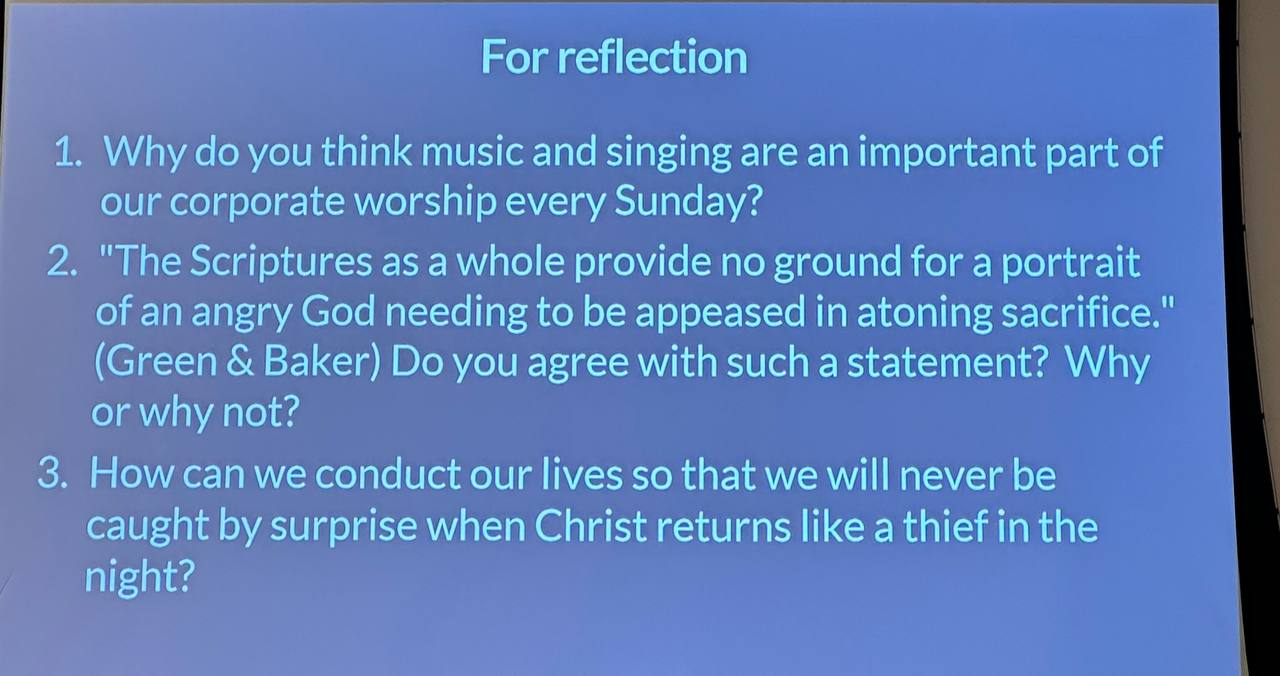
\includegraphics[width=0.8\textwidth, trim={0cm 0cm 0cm 0cm},clip]{Figures/marSermon4Reflections.jpg}
    \includegraphics[width=0.8\textwidth, trim={0cm 0cm 0cm 0cm},clip]{example-image-a}
    \caption[]{Reflection questions for this sermon}
    \label{}
  \end{figure}}
\end{itemize}